%-------------------------------------------------------------------------------
% 
\chapter{Knowledge Acquisition Approach}
%-------------------------------------------------------------------------------

This chapter defines the terms, formal structure and steps that form our 
proposed KA approach. First it introduces the general architecture and 
interaction loop that defines the sequence of interactions and steps
involved in the process(\autoref{section:Architecture}). In the second part, it formalizes 
the upper ontology and logical constructs required for the KA approach 
(\hl{ref to chapter}). After that, each of the crucial steps is described in 
more detail through examples and additions to the core logical structure 
defined earlier.

\section{Architecture}
\label{section:Architecture}
The proposed KA system consists of multiple interconnected technologies and 
functionalities which we grouped into logical modules according to
the problems they are solving (as also defined in \autoref{chapter:background}). 
This was done in order to minimize the complexity, improve the maintenance 
costs and allowing switching the implementations of separate sub-modules. 
Additionally such logical grouping increases the explainability and general
understanding of the system.

\begin{figure}[htb]
	\centering
		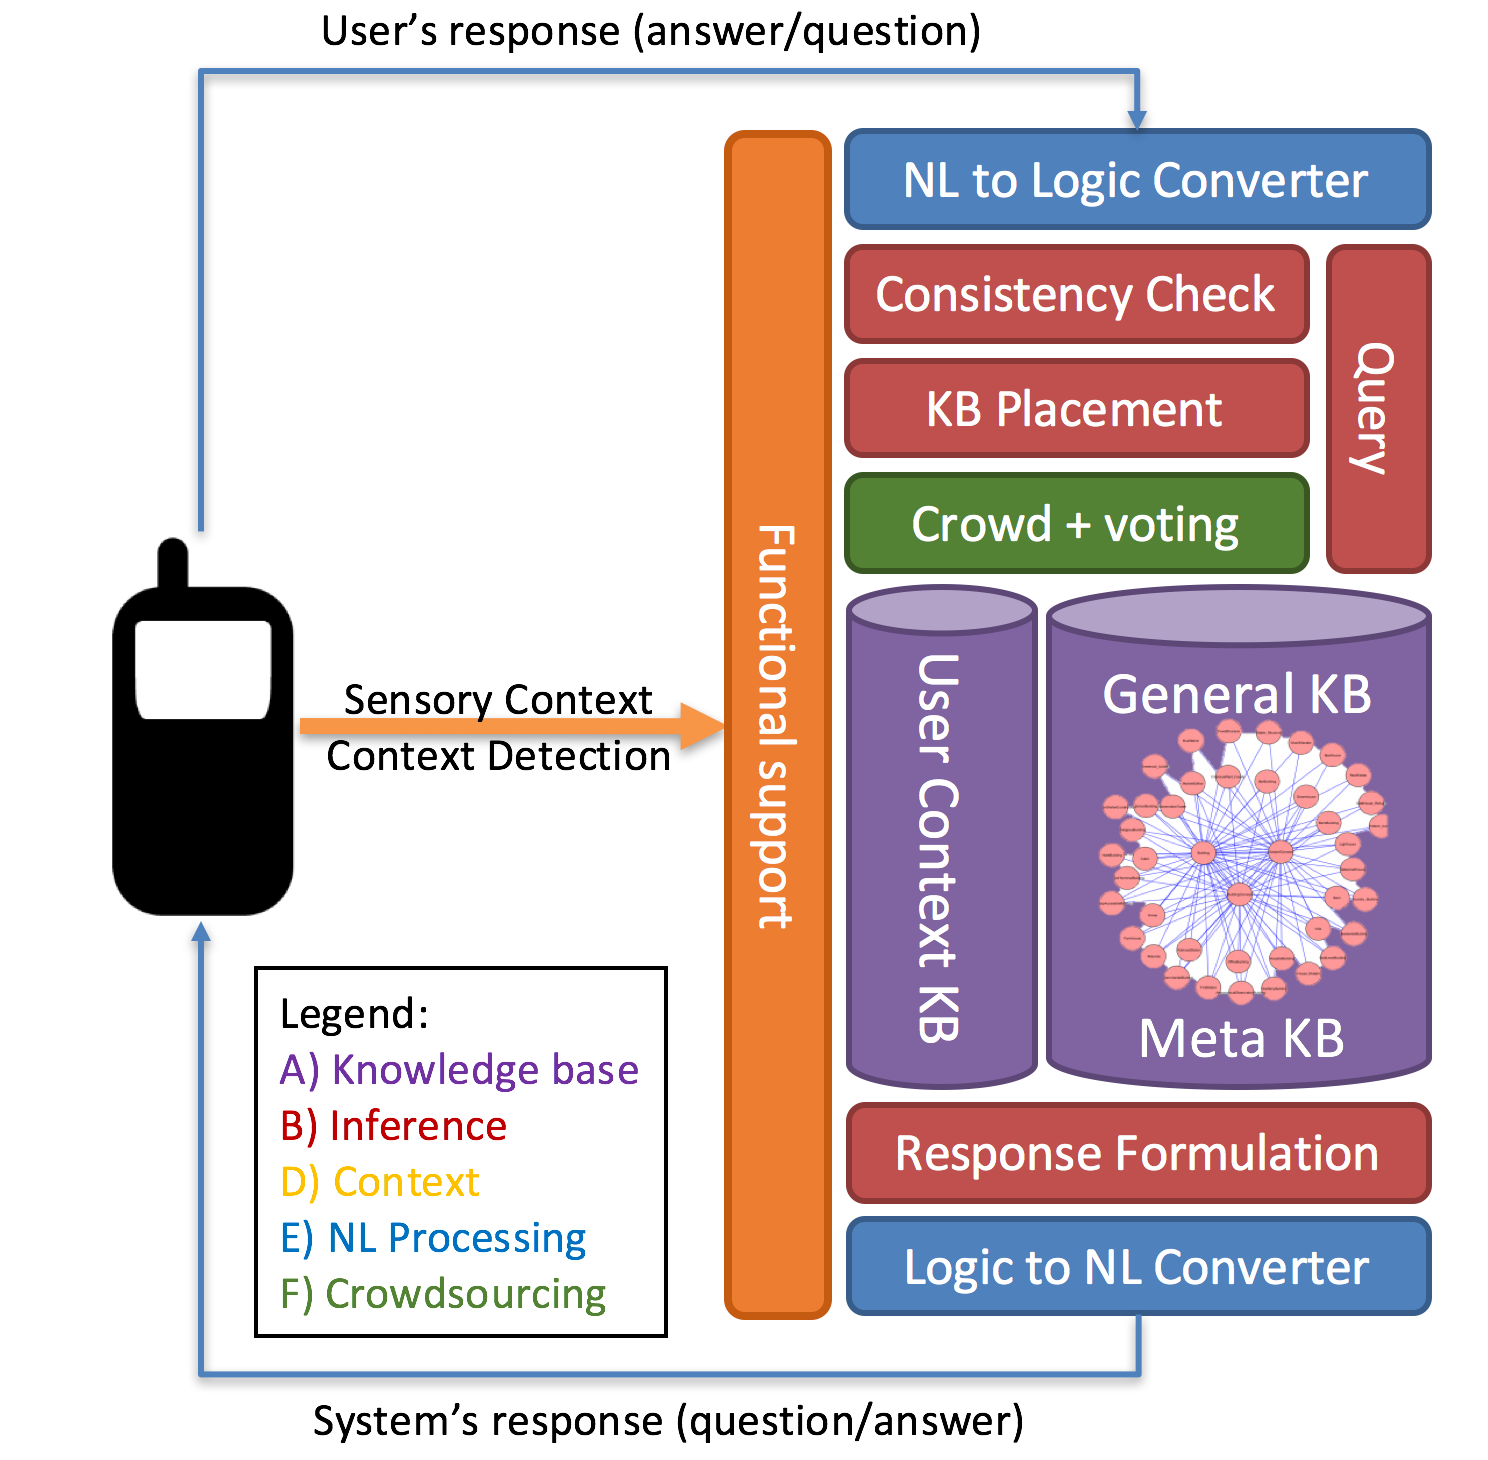
\includegraphics[width=0.9\textwidth]{figures/architecture.png}
	\caption{General Architecture of the KA system, with an interaction loop
			 presented as arrows.}
	\label{fig:Architecture}
\end{figure}


On \autoref{fig:Architecture} these modules are represented with the boxes,
and their functionality groups are presented with the colors (see the figure
legend). Arrows represent the interaction and workflow order and initiation 
(the interaction is initiated/triggered from the origin of the arrow).

We can see that the central core of the
system is the knowledge base (modules marked in purple and letter A). The 
knowledge base consists of \emph{Upper Ontology} gluing everything together, 
\emph{Common Sense Knowledge} to be able to "understand" user's world and check
the answers for consistency, \emph{Meta Knowledge} for enabling inference about 
its internal structures, \emph{User Context KB} to hold current user context and 
\emph{Knowledge Acquisition Rules} to drive the KA process from within the KB, 
using logical inference. 

Next to the KB, is an \emph{Inference Engine} that performs inference over 
the knowledge from the KB. Its modules are represented with the red color 
and letter B. The inference engine needs to be general enough to be able to
perform over full KB, and should be capable of meta-reasoning (over the 
meta-knowledge and KA knowledge in the KB) about the KB's internal knowledge
structures. In cases when the inference engine have some missing functionalities,
some of these tasks can be supplemented by the \emph{Procdeural Support} 
module. In the proposed system, inference engine handles almost all of the 
core KA operations, which can be separated in the following modules:
\begin{itemize}
\item \emph{Consistency Checking} module which can asses the user's answers
and check whether they fit within the current KB knowledge.

\end{itemize}
 for consistency checking
and KB placement of the answer once user provides some knowledge. If the
user is asking a question (as opposed to giving an answer), the inference engine
is used to answer this. And, when in pro-active mode, the questions and 
system's responses are generated by the inference as well (\emph{Response
Formulation} module).

Tightly integrated with the knowledge base and inference engine is a 
\emph{Crowdsourcing Module}, which monitors crowd (multipl user's) answers and 
is able to remove (or move to different contexts) the knowledge from the KB, 
based on its consistency among multiple users. This module is represented in
Green color and letter F.

At the entry and exit point of the system workflow, there are NLP processing  
modules which can convert logic into the natural language and vice versa. These
modules are used for natural language communication with the users. Tese two
modules are represented in Blue and letter E.

On the side of the Figure, there is a procedural module (depicted with Orange
color and letter D), which is a normal software module (in our implementations
written in procedural programming language), which glues everything together.
It contains a web-server, authentication functionalities, machine
learning capabilities, connections to external services and context mining
and other functions that are hard to implement using just logic and inference.
This module is taking care of the interactions between submodules. 

All of the modules are triggered either through the contextual triggers 
(also internal, like when timer detects the specific hour or time of day), or
by the users. When the context changes, it causes the system to use inference
engine to figure out what to do. Usually, as a consequence it results in a 
multiple options like questions or comments. Then it picks one and sends a 
request to the user. This triggering is represented with the arrows, where the 
blue arrows represent natural language interaction, and the orange one
represents structured or procedural interaction, when the procedural module
classifies or detects any useful change in the sensor data sent into the system
py the part running on the mobile phone.

\section{Knowledge Base}
Internally KB has three components. The main part, which should in any real implementation of the system also be the biggest, is the common-sense knowledge and its upper ontology over which we operate. This part of the system contributes the most to the ability to check the answers for consistency. The more knowledge already exists, the easier becomes to assess the answers. The second part is the user Context KB, which stores the contextual knowledge about the user. This covers the knowledge that the user has provided about himself (section 4.4.2) and the knowledge obtained by mining raw mobile sensors (section 4.4.1). This is represented as the orange arrow, pointing into the context part of the KB. The sensor based context allows the system to proactively target the right users at the right time and thus improve the efficiency and accuracy and also stickiness of the KA process.
The third KB part, is the meta-knowledge and KA rules that drive the dialog and knowledge acquisition process (section 4.3.3). Although in our implementation we used Cyc KB and tested Umko KB, the approach is not fixed to any particular knowledge base. But it needs to be expressive enough to be able to cover the intended knowledge acquisition tasks and meta-knowledge needed for the system?s internal workings. 
After the KB, the second most important part of the architecture is an inference engine (in Fig. 2 marked in red and letter B), which is tightly connected to the knowledge base.  The inference engine needs to be able to operate with the concepts, assertions and rules from the KB and should also be capable of meta-reasoning about the knowledge base?s internal knowledge structures. As the individual components (indicated with red color in Fig. 2) suggest, the inference engine is used for:
?	Checking the consistency of the users? answers (e.g., can you order a car in a restaurant if it?s not food?). 
?	Placement of new knowledge inside the KB.
?	Querying the KB to answer possible questions.
?	Using knowledge and meta-rules to produce responses based on the user and her/his context input (similar in function to the scripts in script-based conversational agents).

Fig. 2. General Architecture of the KA system, with a simple interaction loop
At both ends of the stacked chain in Fig. 2, there are natural language processing components (marked in blue and with letter E), which are responsible for logic-to-language and language-to-logic conversion (sections 2.4 and 4.5). These are crucial if we want to interact with users in a natural way and thus avoid the need for users to be experts in first order logic. This module and its components are described in more detail in section 4.5.  
Besides the main interaction loop, which implicitly uses crowdsourcing while it interacts with the users, there is an additional component (marked in green and with letter F). This ?crowdsourcing and voting? component handles and decides, which elements of knowledge (logical assertions) can be safely asserted and made ?visible? to all the users and which are questionable and should stay visible only to the authors of the knowledge. If the piece of knowledge is questionable, the system marks it as such and then the question formulation process will check with other users whether it?s true or not. This is described in more detail in section 4.7.
In addition to logic-based components presented above, there is a functional driver system (marked in orange), which glues everything together, forwards the results of inference to the NL converters, accepts and asserts the context into the KB, handles the synchronization between the instances of the systems, etc.
